\chapter{Related work}\label{sec:rel}
This chapter reviews related work on the \emph{realisability problem} 
for \emph{global types}, both within the same theoretical framework 
and in closely related models.  
The idea of using communicating automata for global types is already 
well established and adopted in various frameworks. Our approach 
adopts an automata-based definition of global types, which captures a 
set of MSCs parameterised by the desired communication semantics.  
This follows the line of research initiated in~\cite{di2023partial} 
and extended in~\cite{di2025realisability}, which aims to establish a 
general framework for communication semantics.  

We have already presented in this thesis the asynchronous 
(\verb|asy|), peer-to-peer (\verb|p2p|), and synchronous 
(\verb|sync|) communication semantics.  
Furthermore, \cite{di2023partial} discusses additional semantics, 
among which the causal order (\verb|co|) and mailbox (\verb|mb|) 
semantics are particularly relevant.
In the causal order model, messages are delivered according 
to their causal dependencies: if $m_1$ causally precedes $m_2$, then 
$m_1$ must be received first~\cite{lamport2019time}.  
Causality, formalised by Lamport’s ``happened-before'' relation, ensures 
consistent delivery order and can be implemented using logical clocks.  
In the mailbox model, all messages sent to the same process, 
regardless of sender, must be received in the order they were sent, 
effectively enforcing FIFO delivery per receiver.  

\cite{di2023partial} also introduces a hierarchy of communication 
semantics, illustrated in a slightly modified form in 
Figure~\ref{fig:coms}.  
The main objective of this work was to establish a hierarchy that 
preserves \emph{monotonic} properties: if a property holds for a given 
communication semantic, it should also hold for all semantics 
contained within it.  
However, it was shown that this monotonicity applies only to specific 
properties, such as \emph{weakly-$k$-synchronisability}~\cite{di2023partial}.  
In contrast, it does not generally extend to the realisability 
problem, which is why we focused on the problem for specific semantics, 
namely peer-to-peer and synchronous communication.

\bigskip

\begin{figure}[!ht]
\centering
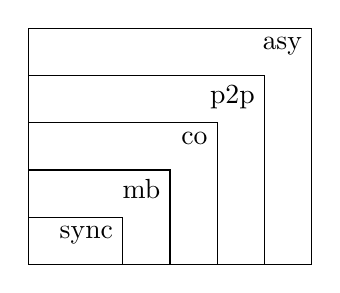
\begin{tikzpicture}[scale=0.6]
  % list of labels in order (from smallest to largest)
%   \def\labels{{rsc,nn,onen,mb,co,p2p,asy}}
  % loop to draw nested squares
  \foreach [count=\i] \lab in {sync,mb,co,p2p,asy} {
    \draw (0,0) rectangle (\i+1,\i);
    \node[anchor=north east] at (\i+1,\i) {\lab};
  }
\end{tikzpicture}
\caption{Hierarchy of communication model semantics.}
\label{fig:coms}
\end{figure}

We then examine recent advances by
Stutz~et~al.~\cite{stutz2024implementability}, who provide a
comprehensive automata-theoretic treatment of the realisability problem,
and trace this line of inquiry back to early results by
Alur~et~al.~\cite{alur2000inference} and
Lohrey~et~al.~\cite{lohrey2003realizability}.  
Finally, we consider formalisms related to Multiparty Session Types
(MPST), such as Choreography Automata~\cite{barbanera2020choreography},
highlighting conceptual connections and key differences with the
approach developed in this thesis.

\section{Realisability of MSCs and HMSCs}
In this section, we compare our framework with one of the earliest and
most influential works on realisability, the one of 
Alur~et~al.~\cite{alur2005realizability}, which also inspired part of our
approach. Their notion of \emph{Weak Realisability} captures the idea that
a specification of Message Sequence Charts (MSCs) should already include
all behaviours that are consistent with the local views of processes. 
Intuitively, a set of MSCs is weakly realisable when, for every process,
the events it observes in any MSC of the specification are compatible
with those in some MSC already in the set. This closure condition ensures
that the global behaviour can be reconstructed from the projections of
individual processes, so that every implied MSC is already part of the
language. 
% Alur~et~al. also provided an equivalent characterisation of
% weak realisability in terms of closure over prefixes of MSCs. 
Our own definition
of weak realisability coincides with theirs, as it expresses the same
fidelity concept over the local behaviour and abstracts from any
deadlock-related concern. In both cases, weak realisability focuses on
the alignment between local and global behaviours rather than on safety
properties such as deadlock-freedom. For safe realisability, we recall an
informal definition of Alur~et~al.~\cite{alur2005realizability} and discuss
the differences.

Intuitively, let $L$ be a set of MSCs. Then $L$ is said to be 
\emph{safely realisable} if there exists a family of communication automata 
$\langle A_i \mid 1 \leq i \leq n \rangle$ such that $L = L(\prod_i A_i)$ 
and the product automaton $\prod_i A_i$ is \emph{deadlock-free}. 
In this setting, a \emph{deadlock state} is a configuration of the global 
system from which no accepting state can be reached. 
This corresponds to a situation where all processes are 
waiting to receive messages that are no longer available in their 
communication buffers, preventing further progress. 
Hence, a system is deadlock-free if no such state is reachable from its 
initial configuration. This notion captures the safety aspect of 
realisability by ensuring that the system never reaches a globally 
stalled state during execution. This definition of safe realisability 
corresponds to ours in $\ppmodel$ or $\synchmodel$.

The work of Alur~et~al.~went on further, defining specific complexity classes 
for different kinds of assumptions. For finite sets of MSCs,
weakly realisability is shown to be \verb|coNP|-complete and safe 
realisability is shown to be decidable in \verb|P|-time. The problem
was subsequently studied for HMSCs. For \emph{bounded} HMSCs, safe realisability 
remains decidable, and it is \verb|EXPSPACE|-complete, but weak realisability 
becomes undecidable. For \emph{unbounded} HMSCs, 
safe realisability remains decidable, and it is \verb|EXPSPACE|-complete, but weak realisability 
becomes undecidable~\cite{alur2005realizability}. 
Later, Lohrey~et al.~\cite{lohrey2003realizability} proved in the general case, 
with a technique that involves five processes, that safe realisability 
is undecidable, though it is decidable (and \verb|EXPSPACE|-complete) 
for a specific kind of HMSCs, called globally-cooperative HMSCs, introducted 
in \cite{morin2002recognizable}.
Furthermore, in the context of weak realisability,
Genest et~al.~\cite{genest2006infinite} introduced the notion of
\emph{locally-cooperative} HMSCs, for which implementability can be
checked in linear time.
Since every globally-cooperative HMSC is also locally-cooperative,
verifying implementability for this broader class remains at least
\verb|EXPSPACE|-hard, if it is decidable at all.
Lohrey~et al.~\cite{lohrey2003realizability} also considered another subclass of HMSC,
called $\mathcal{I}$-closed HMSC, whose checking of safe realisability is \verb|PSPACE|-complete.
Most positive results assume other struttural restrictions, like bounded channels, 
but \cite{bollig2025high} introduces a new class of loop-connected HMSCs
that allows unbounded channels while maintaining realisability.
Table~\ref{tab:realisability-summary} summarises the results presented in this section.

\section{Session Types}
Session Types provide a type-theoretic framework for specifying and verifying 
communication protocols among multiple participants.  
They ensure that interactions follow a predefined structure, 
preventing common concurrency errors such as deadlocks, orphan messages, 
and unspecified receptions. 
Session types were first formalised as 
\emph{Binary Session Types}~\cite{honda1993types}, 
which capture structured communication between two peers.  
The framework later evolved into 
\emph{Multiparty Session Types (MPST)}~\cite{honda2008multiparty}, 
extending the theory to interactions among multiple participants.  
Over the years, session types have been integrated into several programming 
languages~\cite{DBLP:journals/ftpl/AnconaBB0CDGGGH16}, including 
Rust~\cite{jespersen2015session,chen2020ferrite}, 
Haskell~\cite{lindley2016embedding}, 
Erlang~\cite{mostrous2011session}, and
Ocaml~\cite{padovani2017simple}
broadening their practical relevance beyond purely theoretical models.  
They have also found applications across diverse domains such as 
operating systems~\cite{fahndrich2006language}, 
web services~\cite{yoshida2013scribble}, 
distributed algorithms~\cite{kouzapas2024session}, 
and smart contracts~\cite{das2021resource}.  

To sum up, the typical use of MPST involves defining a protocol through 
a \textbf{global type}, from which the \textbf{local types} of each 
participant are derived via a \emph{projection operation}.  
The system implementation, composed of communicating processes, is 
then verified against these local specifications using a 
\emph{typing system}, ensuring safe behaviour and additional properties 
such as deadlock-freedom.
% A key component of classical MPST is the \emph{merge operator}, 
% which resolves non-determinism when projecting away interactions 
% irrelevant to a participant.  
% Since merging is only partially defined, it determines whether local 
% states can be safely combined; when projection succeeds, it guarantees 
% both deadlock freedom and protocol fidelity.  
Figure~\ref{fig:mpstschema} summarises the main elements of this framework.


\begin{figure}[!ht]
\centering
\begin{tikzpicture}[
      node distance=1.2cm,
      every node/.style={font=\sffamily},
      rect/.style={rectangle, draw=black, minimum width=1cm, minimum height=1cm},
      circ/.style={circle, draw=black, minimum size=1cm},
      arrow/.style={-{Stealth[scale=1.1]}, thick}
  ]

  % Nodes
  \node[rect] (G) {\textcolor{red}{$\mathcal{G}$}};
  \node[circ, below=of G] (TB) {\textcolor{blue}{$L_\text{B}$}};
  \node[circ, left=of TB] (TA) {\textcolor{blue}{$L_\text{A}$}};
  \node[circ, right=of TB] (TC) {\textcolor{blue}{$L_\text{C}$}};

  \node[rect, below=of TA] (PA) {\textcolor{brown}{$P_\text{A}$}};
  \node[rect, below=of TB] (PB) {\textcolor{brown}{$P_\text{B}$}};
  \node[rect, below=of TC] (PC) {\textcolor{brown}{$P_\text{C}$}};

  \node[rect,draw=none,right=of TC] (LC) {\textbf{\textcolor{blue}{2. Local type}}};
  \node[rect,draw=none,above=of LC] (LG) {\textbf{\textcolor{red}{1. Global type}}};
  \node[rect,draw=none,below=of LC] (LG) {\textbf{\textcolor{brown}{3. Processes}}};

  % Arrows
  \draw[arrow] (G) -- (TA) node[midway, left] {Projection};
  \draw[arrow] (G) -- (TB);
  \draw[arrow] (G) -- (TC);

  \draw[arrow] (PA) -- (TA) node[midway, left] {Type checking};
  \draw[arrow] (PB) -- (TB);
  \draw[arrow] (PC) -- (TC);
  \draw[arrow] (TC) -- (PC);
  \draw[arrow] (TB) -- (PB);
  \draw[arrow] (TA) -- (PA);

\end{tikzpicture}
\caption{Intuitive schema of MPST framework}
\label{fig:mpstschema}
\end{figure}

\subsection{Projectability}
\emph{Projectability} asks whether a global type can be faithfully 
projected into local specifications for each participant so that the 
resulting local types interact without mismatches or unintended 
behaviours.  
It corresponds to the \emph{realisability} problem studied in 
automata-theoretic settings, both concern whether a global specification 
admits a correct distributed implementation.

However, classical projection algorithms often reject natural yet safe 
protocols because of strong syntactic constraints designed to ensure 
safety.  
This gap between expressiveness and implementability has motivated the 
search for more permissive definitions.  
Notably, the algorithm of Castagna et al.~\cite{castagna2012global} 
was the first to aim for \emph{full completeness}, balancing safety 
and expressiveness.

\subsubsection{Realisability and Restrictions in MPST}
Recent work connects MPST with automata-theoretic models such as High-level 
Message Sequence Charts (HMSCs). Stutz and Zufferey demonstrated that 
realisability is \textbf{decidable} for global types encoded as 
\emph{globally cooperative} HMSCs~\cite{DBLP:journals/corr/abs-2209-10328,DBLP:conf/ecoop/Stutz23}.  
Li et al.~\cite{li2023complete} later introduced a complete projection operator 
ensuring correctness for all implementable global types.  

In his thesis, Stutz~\cite{stutz2024implementability} provides a comprehensive 
classification of the \textbf{syntactic restrictions} that govern both 
\emph{expressiveness} and \emph{decidability} in MPST.  
He generalises the traditional notion of sender-driven choice to allow a sender 
to branch towards different receivers, capturing common distributed patterns 
such as load balancing, while keeping the implementability 
problem \textbf{decidable} in \verb|PSPACE|.  
This establishes the first tight complexity bound for the class of 
sender-driven global types and confirms that they can be faithfully 
represented as HMSCs.  
Note that Stutz~et~al.\ interpret \emph{deadlocks} in the sense of our
\emph{progress} property, and additionally define \emph{soft deadlocks}
for its model.
The latter gives rise to the \emph{soft implementability} problem.

A key syntactic dimension in MPST is how \emph{choice} is handled 
when a branch of the protocol is encountered, as this 
determines whether projection remains decidable.  
The three main variants are:
\begin{itemize}
    \item \emph{Directed choice}: every branch shares the same 
    sender–receiver pair, yielding a single decision point.  
    This ensures safety and straightforward projection but severely limits 
    expressiveness, as many distributed coordination patterns are 
    excluded~\cite{honda2008multiparty}.  

    \item \emph{Sender-driven choice}: each branch has a single sender, 
    but receivers may differ across branches.  
    This generalisation captures richer interaction schemes while retaining 
    decidability; as mentioned, safe realisability for this fragment lies in 
    \verb|PSPACE|~\cite{stutz2024implementability}.  

    \item \emph{Mixed choice}: multiple senders may initiate branches 
    concurrently, removing a unique decision-maker.  
    While this maximises expressiveness, it introduces intrinsic 
    nondeterminism in control flow, making implementability and its 
    weaker variants (e.g., soft or weak realisability) \textbf{undecidable} 
    in general~\cite{stutz2024implementability}.  
\end{itemize}

These results precisely delineate the boundary between expressiveness and 
decidability in MPST.  
Stutz’s framework provides the first complete algorithmic account of 
implementability for sender-driven global types and proves that no 
complete algorithm can exist once mixed choice is permitted.


\section{Choreographies}
Choreographies \cite{ws-cdl-2005} and Choreographic 
Programming~\cite{montesi2014choreographic, giallorenzo2024choral, cruz2022functional} 
are other formalisms to describe  
distributed communication protocols. Choreographies emphasize the 
global specification of interactions as a high-level description of the 
intended message exchanges. Similarly to MPST, their goal is to ensure that
a distributed implementation can be derived in which each participant 
follows a local behaviour consistent with the global description, called
respectively \emph{local} and \emph{global}-view. This setting naturally 
connects to the realisability problem, since the key question is whether 
a choreography can be faithfully implemented by a system of local 
processes. 
In choreographies, the local-view is called 
\textbf{End-Point Projection} (EPP),
and it is derived via a projection operation from the global-view.
In particular, \emph{Choreography Automata}~\cite{barbanera2020choreography}  
share many conceptual similarities with our notion of Global Types.  
Both formalisms model global interaction structures through automata  
over communication actions, capturing the causal dependencies among  
participants. The main difference lies in the underlying semantics and  
the intended use: Choreography Automata focus on synthesis and  
verification within choreographic frameworks, while our Global Types  
are tailored to the study of realisability under different
communication semantics.  

One important challenge studied in choreographic design is the 
\textbf{knowledge of choice} problem~\cite{lanese2008bridging, castagna2012global}. 
This problem can be seen as a 
specific instance of the general projection problem: it arises when 
translating a global description into consistent local behaviours. 
In particular, it captures the difficulty of maintaining coherence 
when decisions made by one participant must be known by others.  

Informally, a choreography has knowledge of choice if, whenever a 
branching (conditional) decision is made by one participant, all 
other affected participants are made aware of that decision. Without 
proper communication of the choice, a participant may behave 
inconsistently because it lacks information to distinguish which 
branch was taken. For example, if process \(A\) chooses between two 
branches that lead to different sub-protocols with process \(B\), 
then \(B\) must receive a signal (a ``selection'') that lets it 
synchronize on the correct continuation.  

If the choreography lacks such a mechanism, it becomes 
\emph{unprojectable}: EPP is not allowed to generate local behaviours 
that coordinate the branching uncorrectly. This issue 
is addressed, typically, by adding explicit selection messages to 
propagate the choice, and how this can be automated via 
\emph{amendment} or \emph{repair} algorithms 
\cite{DBLP:journals/corr/LaneseMZ13, basu2016automated}, 
which insert minimal extra 
communications to guarantee knowledge of choice.  

Conceptually, this problem is closely related to the \emph{sender-driven 
choice} policy highlighted before in the MPST framework, where 
multiple senders make independent choices that must be reconciled to 
ensure a coherent global behaviour. In both cases, the challenge lies 
in ensuring that all participants have sufficient knowledge to follow 
the same branch, preserving consistency across local projections. 


\section{Other works}
In his thesis~\cite{stutz2024implementability}, 
Stutz further investigate which syntactic and semantic
restrictions in global types are \emph{non-restrictive}, that is, those that
do not compromise expressiveness while preserving decidability.  
Stutz et al.~introduce
\emph{Protocol State Machines} (PSMs)~\cite{stutz2025automata}, 
a unifying automata-theoretic
formalism that strictly generalises both Global Types and HMSCs.  
This model captures interaction protocols as communicating state
machines over message-passing labels, bridging automata theory and MPST.
His results show that every sink-final $\Sigma 1$-PSM can be represented
as a non-deterministic Global Type that preserves sender-driven or
mixed-choice behaviour~\cite[Thm.~8.14]{stutz2024implementability}.  
Later, Stutz et~al.~\cite{stutz2025automata} extended this line of work,
formalising PSMs and analysing the computational complexity of type
checking and realisability. They demonstrate that, for choice-free or
single-choice fragments, both problems remain decidable (often in
\verb|PTIME|), whereas the introduction of \emph{mixed choice} renders
realisability \emph{undecidable}.  
Together, these results reinforce the view that structural constraints
such as single recursion points or explicit termination are
\emph{expressively harmless}, while the distinction between
\emph{sender-driven} and \emph{mixed} choice constitutes the true
boundary between decidability and undecidability in distributed protocol
implementations.

Another relevant contribution is by Guanciale et al.~ 
\cite{DBLP:journals/jlap/GuancialeT19}, who study the 
\emph{realisability of pomsets} via communicating automata. 
Pomsets, or partially ordered multisets, generalise MSCs by 
capturing causal dependencies among events rather than total 
orders. Their work defines realisability conditions ensuring 
both communication correctness and termination soundness, 
supporting participants with internal concurrency.
Table~\ref{tab:realisability-summary} summarises the 
main results analised in the last sections. To our knowledge, 
empty cells are to be considered open problems, like
the safe realisability problem for sender-driven HMSCs
and PSMs.

\bigskip

\begin{table}[!ht]
\centering
\renewcommand{\arraystretch}{1.3}
\begin{tabular}{|p{4.3cm}|p{4.3cm}|p{4.3cm}|}
\hline
\textbf{Formal Model} & \textbf{Weak Realisability} & \textbf{Safe Realisability} \\ 
\hline
\textbf{Finite sets of MSCs} 
& coNP-complete~\cite{alur2005realizability} 
& P-time~\cite{alur2005realizability} \\ 
\hline
\textbf{Unbounded HMSCs} 
& Undecidable~\cite{lohrey2003realizability} 
& Undecidable~\cite{lohrey2003realizability} \\ 
\hline
\textbf{Bounded HMSCs (FIFO)} 
& Undecidable~\cite{alur2005realizability} 
& EXPSPACE-complete~\cite{lohrey2003realizability} \\ 
\hline
\textbf{Bounded HMSCs (non-FIFO)} 
& Decidable~\cite{morin2002recognizable} 
& EXPSPACE-complete~\cite{lohrey2003realizability} \\ 
\hline
\textbf{Globally-Cooperative HMSCs} 
& -- 
& EXPSPACE-complete~\cite{morin2002recognizable} \\ 
\hline
\textbf{Locally-Cooperative HMSCs} 
& Linear time~\cite{genest2006infinite}
& At most EXPSPACE-complete~\cite{morin2002recognizable}  \\ 
\hline
\textbf{$\mathcal{I}$-Closed HMSCs} 
& -- 
& PSPACE-complete~\cite{lohrey2003realizability} \\ 
\hline
\textbf{Loop-connected HMSCs (unbounded channels)} 
& Decidable~\cite{bollig2025high}
& -- \\ 
\hline
\textbf{MPST (directed choice)} 
& --
& Decidable, but incomplete~\cite{honda2008multiparty} \\ 
\hline
\textbf{MPST (sender-driven choice)} 
& --
& PSPACE-complete~\cite{stutz2024implementability} \\ 
\hline
\textbf{MPST (mixed choice)} 
& Undecidable~\cite{stutz2024implementability} 
& Undecidable~\cite{stutz2024implementability} \\ 
\hline
\textbf{General PSMs} 
& --
& Undecidable~\cite{stutz2025automata} \\ 
\hline
\textbf{Choreographic Programming} 
& --
& Decidable~\cite{barbanera2020choreography} \\ 
\hline
\end{tabular}
\caption{Summary of computational complexity for weak and safe realisability across formal models.}
\label{tab:realisability-summary}
\end{table}

\section{Related Tools}\label{sec:reltool}
Several verification tools have been developed to analyse communicating 
automata and distributed systems under asynchronous or bounded communication 
semantics. 

\textsc{McScM}~\cite{heussner2012mcscm} is the tool most closely related 
to \textsc{ReSCu}. It takes as input a system description and a set of 
\emph{bad configurations} (expressed using Queue Decision Diagrams, QDDs, 
from~\cite{boigelot1996symbolic}) and checks their reachability. 
The tool implements multiple model-checking strategies based on abstract 
interpretation~\cite{cousot1977abstract} and supports general classes of communicating systems.  
In contrast to \textsc{ReSCu}, most approaches in \textsc{McScM} are 
\emph{semi-algorithms}, requiring user-defined timeouts to terminate.  
However, its strength lies in providing a diverse set of verification 
engines, which increases the likelihood of obtaining conclusive verification 
results.  
Notably, \textsc{ReSCu} reuses the same input description language as 
\textsc{McScM}, ensuring compatibility and easing system specification.

\textsc{KMC}~\cite{lange2019verifying} (for \emph{k-Multiparty 
Compatibility}) was introduced by Lange and Yoshida to verify whether a 
system could have been derived from a \emph{Multiparty Session Type} (MPST).  
If a system satisfies $k$-MC, several safety properties, such as freedom from 
deadlock and orphan messages, are guaranteed automatically.  
Unlike \textsc{ReSCu} and \textsc{McScM}, \textsc{KMC} does not require the 
explicit specification of safety conditions but relies on the theoretical 
guarantees of MPST projection.

The \textsc{STaB-C} tool~\cite{akroun2018automated,akroun2016automated} 
implements semi-algorithms for checking \emph{k-stability}, a property that 
guarantees behavioural equivalence across different communication bounds.  
A system is $k$-stable if, for any larger bound $k' > k$, its behaviour 
remains equivalent (under various notions of trace or observational 
equivalence).  
While \textsc{STaB-C} focuses on detecting stability rather than verifying 
safety or liveness, it provides important insight into boundedness and 
behavioural robustness of FIFO systems.  
Unlike \textsc{ReSCu}, which verifies multiple semantic properties such as 
deadlock-freedom and progress, \textsc{STaB-C} focuses exclusively on 
membership in the class of $k$-stable systems.
